% GNSS-Disciplined Cuckoo Clock: project description
% Typeset from docs/project-description.html; the text follows that page.
% Build: latexmk -pdf project-description.tex
\documentclass[11pt,letterpaper]{article}

\usepackage[T1]{fontenc}
\usepackage[utf8]{inputenc}
\usepackage{XCharter}
\usepackage[scale=0.92]{sourcesanspro}
\usepackage[scaled=0.85]{beramono}
\usepackage{microtype}
\usepackage[margin=1in,headheight=14pt]{geometry}
\usepackage{xcolor}
\usepackage{graphicx}
\usepackage{booktabs,tabularx,array}
\usepackage{enumitem}
\usepackage[font={small,sf},labelfont={bf},labelsep=period,
            justification=raggedright,singlelinecheck=false]{caption}
\usepackage{titlesec}
\usepackage{fancyhdr}
\usepackage{tikz}
\renewcommand{\topfraction}{0.85}\renewcommand{\textfraction}{0.1}\renewcommand{\floatpagefraction}{0.75}
\usetikzlibrary{arrows.meta}
\usepackage[hidelinks]{hyperref}

\graphicspath{{../figures/}}

% Colors from the web page's light theme
\definecolor{ink}{HTML}{1C2230}
\definecolor{quiet}{HTML}{5A6272}
\definecolor{axis}{HTML}{9AA1AD}
\definecolor{rule}{HTML}{DDE1E7}
\definecolor{accent}{HTML}{2B5FB4}
\color{ink}

\hypersetup{
  pdftitle={GNSS-Disciplined Cuckoo Clock: An Interdisciplinary Senior Design Project},
  pdfauthor={Nathaniel Frissell, W2NAF},
  pdfsubject={Senior design project description},
  pdfkeywords={GNSS, PPS, Shortt clock, Shakespeare Programming Language, punched cards, W3USR}
}

\titleformat{\section}{\sffamily\Large\bfseries\color{ink}}{}{0pt}{}
\titlespacing*{\section}{0pt}{2.2ex plus .5ex minus .2ex}{0.9ex}

\setlist{itemsep=0.35ex, topsep=0.6ex}
\setlist[itemize]{label=\textcolor{axis}{\textbullet}, leftmargin=1.4em}
\setlist[enumerate]{leftmargin=1.8em}

\pagestyle{fancy}
\fancyhf{}
\renewcommand{\headrulewidth}{0pt}
\fancyhead[R]{\sffamily\footnotesize\color{quiet}GNSS-Disciplined Cuckoo Clock}
\fancyfoot[C]{\sffamily\footnotesize\color{quiet}\thepage}
\fancypagestyle{plain}{\fancyhf{}\fancyfoot[C]{\sffamily\footnotesize\color{quiet}\thepage}}

\setlength{\parskip}{0.55ex plus 0.2ex}
\setlength{\parindent}{0pt}
\renewcommand{\arraystretch}{1.25}
\newcolumntype{L}[1]{>{\raggedright\arraybackslash}p{#1}}
\newcolumntype{Y}{>{\raggedright\arraybackslash}X}

\newcommand{\lead}[1]{\textbf{#1}}

% Diagram styles, drawn in the SVG's pixel coordinates (y down)
\tikzset{
  dia/.style={x=0.0085in, y=-0.0085in, font=\sffamily, line width=0.8pt,
    >={Stealth[length=6.5pt,width=5pt]}},
  box/.style={draw=axis, rounded corners=3pt},
  conn/.style={draw=axis, ->},
  note/.style={font=\sffamily\scriptsize, text=quiet},
}
% \blk{x}{y}{title}{subtitle}: a 160 x 56 box with its top-left corner at (x,y)
\newcommand{\blk}[5][box]{%
  \draw[#1] (#2,#3) rectangle ++(160,56);
  \node[font=\sffamily\footnotesize\bfseries] at (#2+80,#3+21) {#4};
  \node[note] at (#2+80,#3+38) {#5};}

\begin{document}

\thispagestyle{plain}
\begin{flushleft}
{\sffamily\bfseries\LARGE GNSS-Disciplined Cuckoo Clock:\\[0.3ex]
 \Large An Interdisciplinary Senior Design Project\par}
\vspace{1.2ex}
{\sffamily\color{quiet} Nathaniel Frissell, W2NAF, University of Scranton\quad\textbullet\quad
 October 28, 2026\par}
\vspace{1ex}
{\color{rule}\rule{\textwidth}{0.6pt}}
\end{flushleft}

\begin{figure}[h]
  \centering
  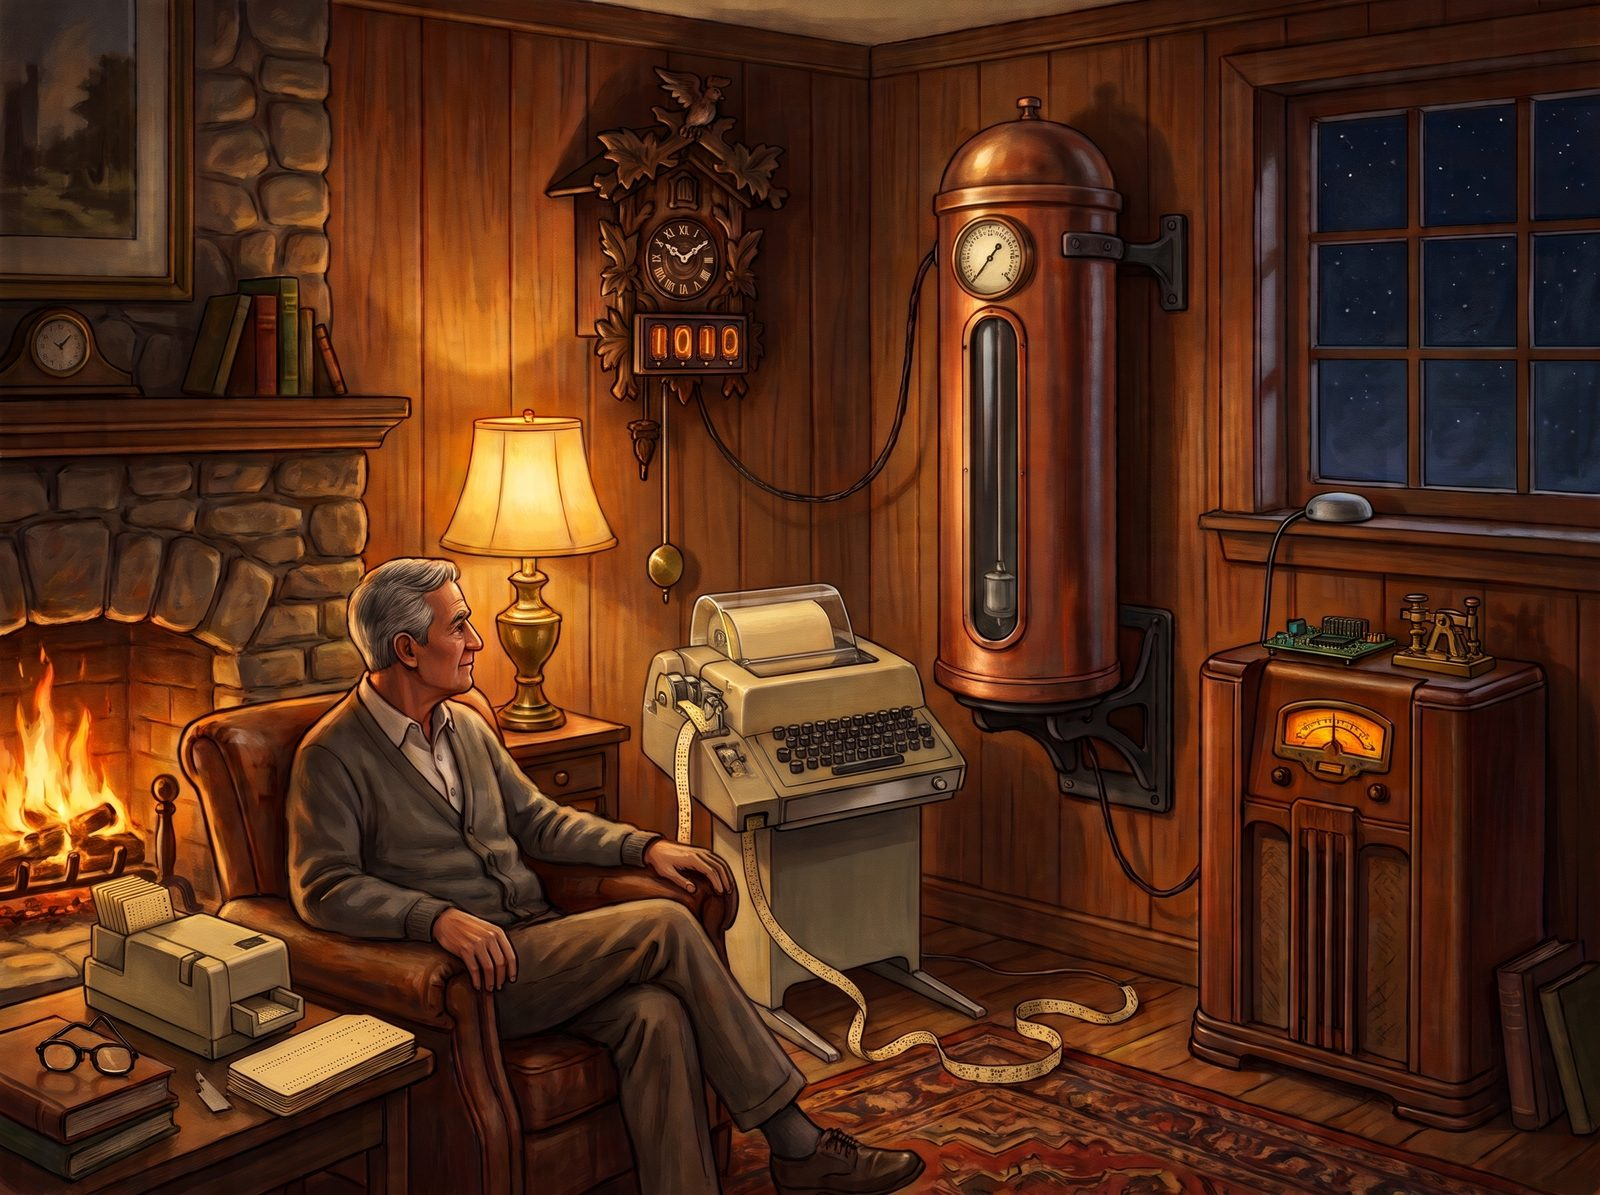
\includegraphics[width=\textwidth]{clock-at-home.jpg}
  \caption*{The finished clock at home: the Shortt-style master in its vacuum tank driving
    the cuckoo's slave pendulum, Nixie and dial agreeing on the time, the Teletype console,
    the card reader, and the GNSS antenna and WWV receiver. \textit{(Illustration.)}}
\end{figure}

\section{Project overview}

Students will build a mechanical cuckoo clock whose timekeeping is disciplined to GNSS,
running control firmware written in the Shakespeare Programming Language (SPL) and loaded
from punched cards. The cards are produced by a microcontroller-driven card punch, fed by an
AI translation stage that converts a reference implementation written in Rust into SPL.

GNSS, short for Global Navigation Satellite System, is the general term for satellite
navigation systems. The United States' GPS is the best known, alongside Europe's Galileo,
Russia's GLONASS, and China's BeiDou. Each satellite broadcasts its position and a time signal
derived from onboard atomic clocks, so a receiver that hears four or more satellites can solve
for both its location and the exact time. A timing receiver turns that solution into a
pulse-per-second (PPS) output aligned to Coordinated Universal Time (UTC), and that pulse is
the reference this clock is disciplined to. Using all four systems rather than GPS alone keeps
the clock locked when the sky view is poor or one system has an outage.

The project deliberately chains together four eras of computing: 18th-century clockwork,
1960s punched-card media, modern satellite timing, and present-day machine translation of
code. Each link in the chain is a real engineering problem, and each hand-off between links is
an interface the teams must specify, test, and defend.

The absurdity is the point, but it is load-bearing absurdity. An esoteric target language
forces rigorous verification of AI-generated code. A physical card medium forces students to
think about encoding, error detection, and data integrity. A pendulum that must track GNSS to
the second forces a real control-loop design rather than a software clock that simply resets
itself.

The project is intended for a two-semester senior design sequence with a team of roughly
6--9 students drawn from electrical engineering, mechatronics, and computer science.

\section{System architecture}

The build path runs one way from Rust source to a punched deck; the only feedback loops are
the test gate that rejects bad translations and the clock's own discipline loop.

\begin{figure}[!htbp]
\centering
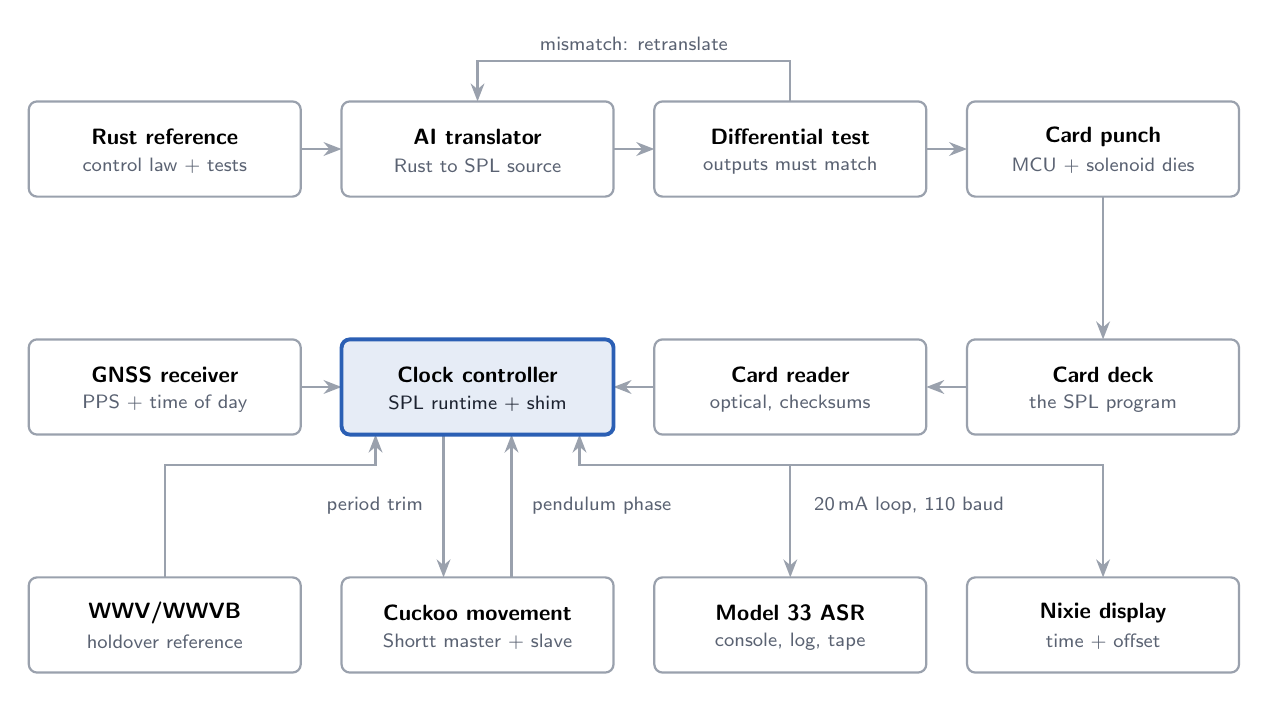
\begin{tikzpicture}[dia]
  % connectors
  \draw[conn] (184,128) -- (208,128);
  \draw[conn] (368,128) -- (392,128);
  \draw[conn] (552,128) -- (576,128);
  \draw[conn] (472,100) -- (472,76) -- (288,76) -- (288,100);
  \node[note] at (380,66) {mismatch: retranslate};
  \draw[conn] (656,156) -- (656,240);
  \draw[conn] (576,268) -- (552,268);
  \draw[conn] (392,268) -- (368,268);
  \draw[conn] (184,268) -- (208,268);
  \draw[conn] (268,296) -- (268,380);
  \draw[conn] (308,380) -- (308,296);
  \node[note, anchor=east] at (262,338) {period trim};
  \node[note, anchor=west] at (314,338) {pendulum phase};
  \draw[conn] (104,380) -- (104,314) -- (228,314) -- (228,296);
  \draw[conn] (472,314) -- (656,314) -- (656,380);
  \draw[draw=axis, <->] (348,296) -- (348,314) -- (472,314) -- (472,380);
  \node[note, anchor=west] at (480,338) {20\,mA loop, 110 baud};
  % build path
  \blk{24}{100}{Rust reference}{control law + tests}
  \blk{208}{100}{AI translator}{Rust to SPL source}
  \blk{392}{100}{Differential test}{outputs must match}
  \blk{576}{100}{Card punch}{MCU + solenoid dies}
  % clock
  \blk{24}{240}{GNSS receiver}{PPS + time of day}
  \blk[draw=accent, line width=1.4pt, fill=accent!12, rounded corners=3pt]{208}{240}%
      {Clock controller}{\color{ink}SPL runtime + shim}
  \blk{392}{240}{Card reader}{optical, checksums}
  \blk{576}{240}{Card deck}{the SPL program}
  \blk{24}{380}{WWV/WWVB}{holdover reference}
  \blk{208}{380}{Cuckoo movement}{Shortt master + slave}
  \blk{392}{380}{Model 33 ASR}{console, log, tape}
  \blk{576}{380}{Nixie display}{time + offset}
\end{tikzpicture}
\caption{System architecture: build path and clock loop. Rust becomes punched SPL cards that
  steer a GNSS-locked pendulum.}
\label{fig:architecture}
\end{figure}

The controller compares each GNSS pulse-per-second edge with the pendulum's optical gate, and
the SPL program turns that phase error into a period trim. The punch-and-read path is offline:
cards are punched once per firmware build and read at boot.

\section{Subsystems and team responsibilities}

The system divides into six subsystems, each with a lead discipline and at least one
supporting discipline so that no team works in isolation.

\begin{table}[!htbp]
\small
\begin{tabularx}{\textwidth}{@{}L{1.55in}L{0.9in}L{0.85in}Y@{}}
\toprule
\sffamily\bfseries Subsystem & \sffamily\bfseries Lead discipline
  & \sffamily\bfseries Supporting & \sffamily\bfseries Core tasks \\
\midrule
1.~Rust reference firmware & CS & EE &
  Write the GNSS-discipline algorithm (PPS phase measurement, PI loop, chime scheduling) in
  Rust; build a test suite and simulator \\
2.~AI Rust-to-SPL translator & CS & --- &
  Prompting/tooling to translate Rust to SPL; automated equivalence testing against the Rust
  reference \\
3.~Card encoder and punch & Mechatronics & EE, CS &
  Define a card encoding for SPL source; design and build a microcontroller-driven punch
  (solenoid or stepper die actuation, card feed, registration) \\
4.~Card reader & EE & Mechatronics &
  Optical (LED/phototransistor array) or mechanical card reader with checksum validation;
  streams program into the clock controller \\
5.~Clock controller and SPL runtime & EE & CS &
  Microcontroller board with GNSS receiver, PPS capture, and an SPL interpreter or
  spl2c-compiled image with a hardware I/O shim \\
6.~Cuckoo mechanism and discipline actuator & Mechatronics & EE &
  Shortt-style free master pendulum in a sealed tank, slave pendulum with hit-and-miss
  synchronizer, optical gate sensing, master rate trim, cuckoo bird and bellows drive,
  hour/half-hour strike \\
\bottomrule
\end{tabularx}
\caption{Subsystems, lead and supporting disciplines, and core tasks.}
\label{tab:subsystems}
\end{table}

CS students own correctness of the code path from Rust to SPL. Mechatronics students own
everything that moves. EE students own timing, sensing, power, and the board-level
electronics that tie the other two together.

\section{Model 33 Teletype console}

A Model 33 ASR Teletype serves as the clock's operator console, its log printer, and a
paper-tape fallback for the card path. Mechatronics restores it, EE builds the interface, and
CS writes the console protocol.

\begin{itemize}
  \item \lead{Console and log:} the controller prints one line per hour (GNSS time, pendulum
    phase error, trim command) and accepts typed commands such as status or forced holdover.
    The clock's discipline performance accumulates on a paper roll.
  \item \lead{Program listings:} before a deck is punched, the SPL source prints on the
    Teletype for human review, giving every build a hard-copy listing.
  \item \lead{Paper-tape fallback:} the ASR's tape punch and reader give a second,
    period-correct program medium if the card punch or reader slips.
  \item \lead{Interface:} the 33 speaks a 20\,mA current loop at 110 baud with two stop bits,
    not RS-232 levels. EE builds an optoisolated current-loop-to-UART adapter with its own
    loop supply.
\end{itemize}

Constraints to plan around: the 33 prints uppercase only, at about 10 characters per second,
so a long SPL listing takes a while (tape keeps full ASCII, so case survives on tape). It
needs cleaning and lubrication before reliable service. Its character timing comes from a
synchronous AC motor, so its baud clock follows mains frequency, not GNSS; timing its start
bits against PPS could make a crude grid-frequency monitor as a side experiment.

\begin{figure}[!htbp]
  \centering
  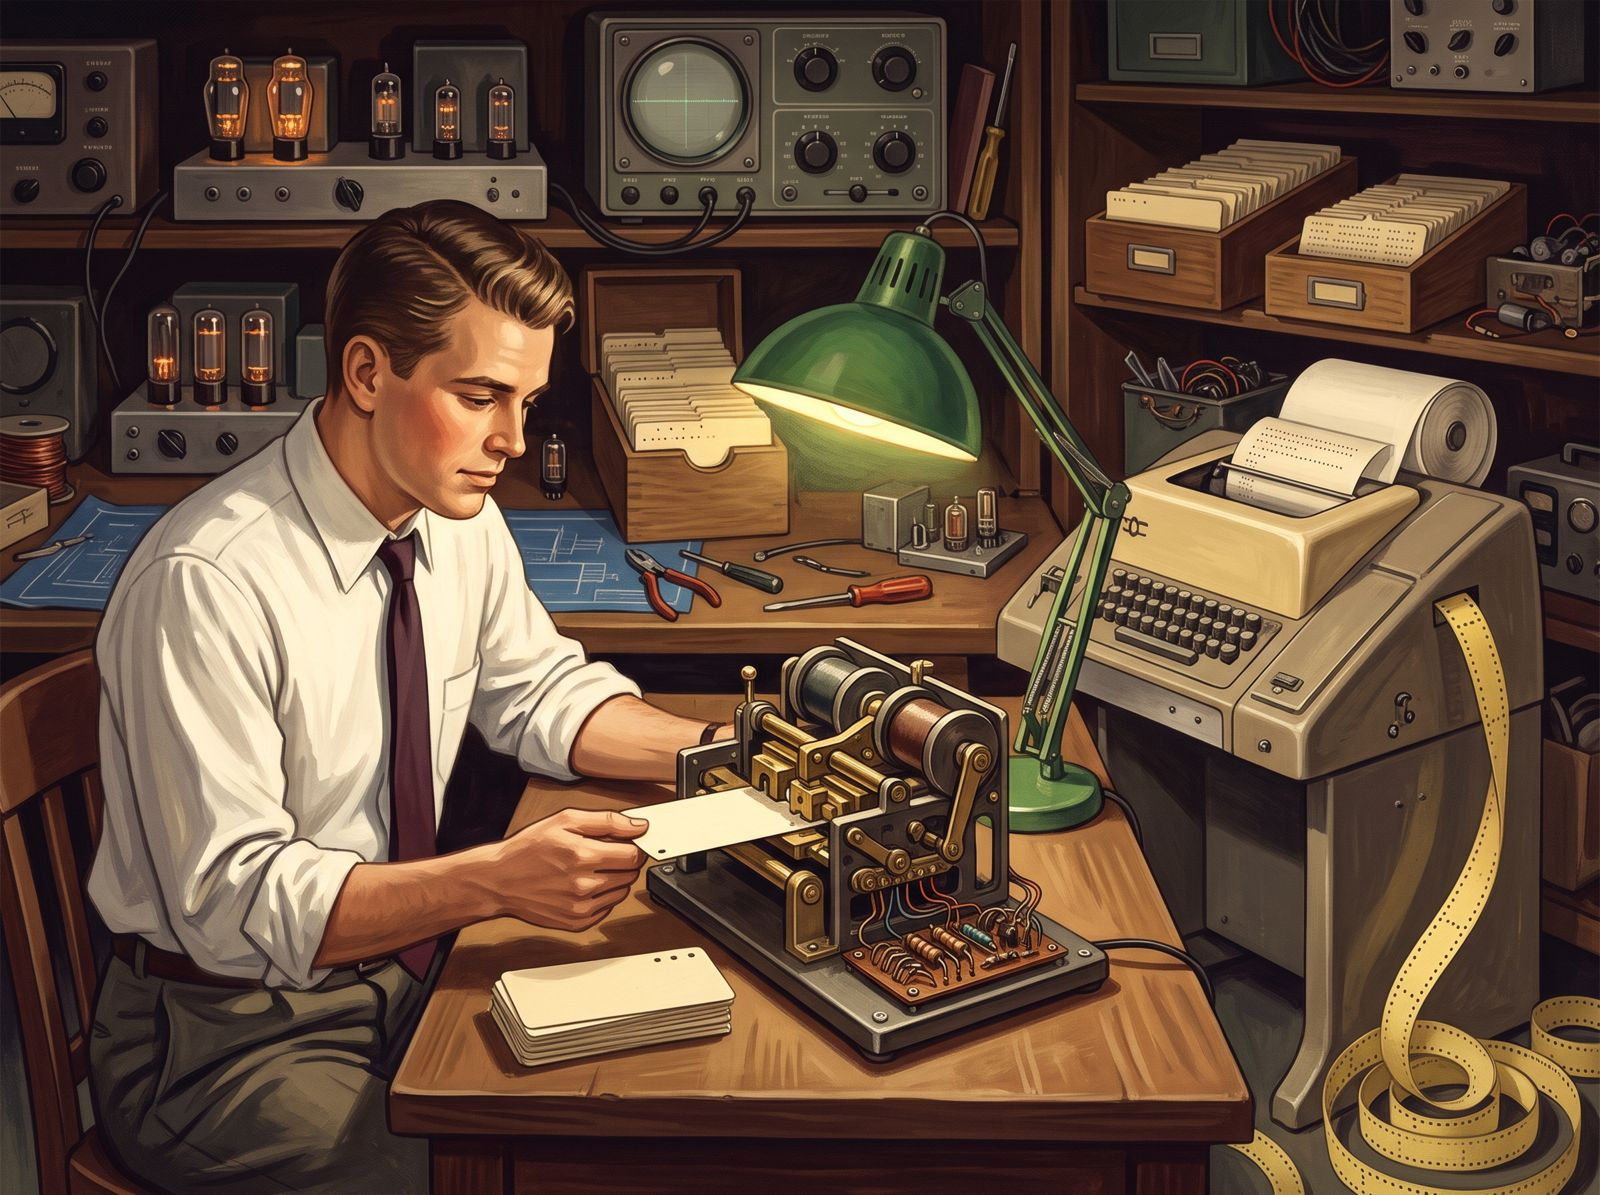
\includegraphics[width=0.8\textwidth]{card-punch-and-teletype.jpg}
  \caption{The card punch and the Teletype console: one makes the program, the other prints
    its listing and the clock's log. \textit{(Illustration.)}}
\end{figure}

\section{Additional features}

Four additions give each discipline one more visible piece: a second time reference, an
audible time announcement, a display, and an optional constellation experiment.

\begin{itemize}
  \item \lead{WWV/WWVB second reference (EE lead):} a 60\,kHz WWVB receiver, or an SDR tuned
    to WWV on HF, gives the controller an independent reference. During a GNSS outage,
    holdover is measured against WWV/WWVB instead of free-running, and the two references can
    be logged side by side. Radio propagation delay limits this to millisecond-class accuracy,
    which is still far finer than a pendulum needs.
  \item \lead{Morse time announcement (CS lead):} after the cuckoo calls the hour, the time is
    sent in CW on a sounder and printed on the Teletype. The Morse encoder is written in Rust
    and goes through the same translate-test-punch path, so it ships in SPL like everything
    else.
  \item \lead{Nixie display (EE and mechatronics):} GNSS time on Nixie tubes beside the
    pendulum, with a small readout of the current clock offset so visitors can watch the loop
    work. The tubes need a high-voltage supply of roughly 170\,V\,DC, which the safety plan
    must cover.
  \item \lead{Constellation comparison (EE and CS, optional):} each constellation keeps its
    own system time: GPS Time, Galileo System Time, BeiDou Time, and GLONASS time tied to
    UTC(SU). The receiver reconciles them and steers PPS to UTC, but students can also log
    each system's timing solution separately and compare offsets and stability across the
    multi-day runs. A dual-frequency timing receiver adds a second experiment: measuring how
    much ionospheric-delay correction improves timing.
\end{itemize}

\section{Technical challenges and open questions}

The hardest problems sit at the interfaces, not inside the subsystems.

\begin{itemize}
  \item \lead{SPL has no hardware access.} The language reads and writes characters and
    integers on standard I/O and nothing else. The runtime must map that stream onto
    hardware: for example, the SPL program reads PPS-to-pendulum phase error as an integer
    and writes a trim command as an integer, with a C or Rust shim handling the actual
    peripherals. Teams must decide how much logic lives in SPL versus the shim, and the
    grading rubric should require that the control law itself is in SPL.
  \item \lead{SPL runtime on a microcontroller.} The common spl2c translator emits C that can
    be cross-compiled, but it is not designed for embedded targets. A small purpose-built SPL
    interpreter may be easier to fit and to feed from a card reader.
  \item \lead{Trusting AI-translated code.} LLM translation into an esoteric language will
    produce plausible but wrong programs. The translator team needs a differential testing
    harness that runs the Rust reference and the SPL output on identical recorded phase-error
    sequences and requires matching outputs before anything is punched.
  \item \lead{Card encoding and program size.} SPL is extremely verbose; a modest control loop
    may run to thousands of lines. At 80 columns per card, card count and reader reliability
    become real constraints. Options include a compact token encoding, a per-card sequence
    number, and per-card checksums.
  \item \lead{The reader is not optional.} The brief specifies punching cards, but the clock
    must also read them. That reader is a full subsystem and should be scoped from the start.
  \item \lead{Disciplining a pendulum.} A mechanical pendulum's period drifts with temperature
    and amplitude. The discipline loop must estimate phase against GNSS PPS and steer the
    period through a small actuator, with loop time constants of minutes, not milliseconds.
    Holdover behavior when GNSS is lost should be specified.
  \item \lead{Movement: a Shortt--Synchronome-style free pendulum.} The clock uses a Shortt
    master-and-slave pair instead of an ordinary cuckoo pendulum. A free master pendulum
    swings in a sealed, partially evacuated tank, receives an impulse every 30 seconds, and
    does no other work. A slave pendulum drives the cuckoo movement and is kept in step by the
    classic hit-and-miss synchronizer. GNSS disciplines the master through a very small rate
    trim, so the system nests two loops: the 1920s mechanical bang-bang loop inside a modern
    PI loop. Students build a replica, not a restored original, since surviving Shortt clocks
    are rare museum pieces. The master's tank, invar rod, and impulse mechanism will be the
    largest mechatronics task in the project.
\end{itemize}

\begin{figure}[!htbp]
  \centering
  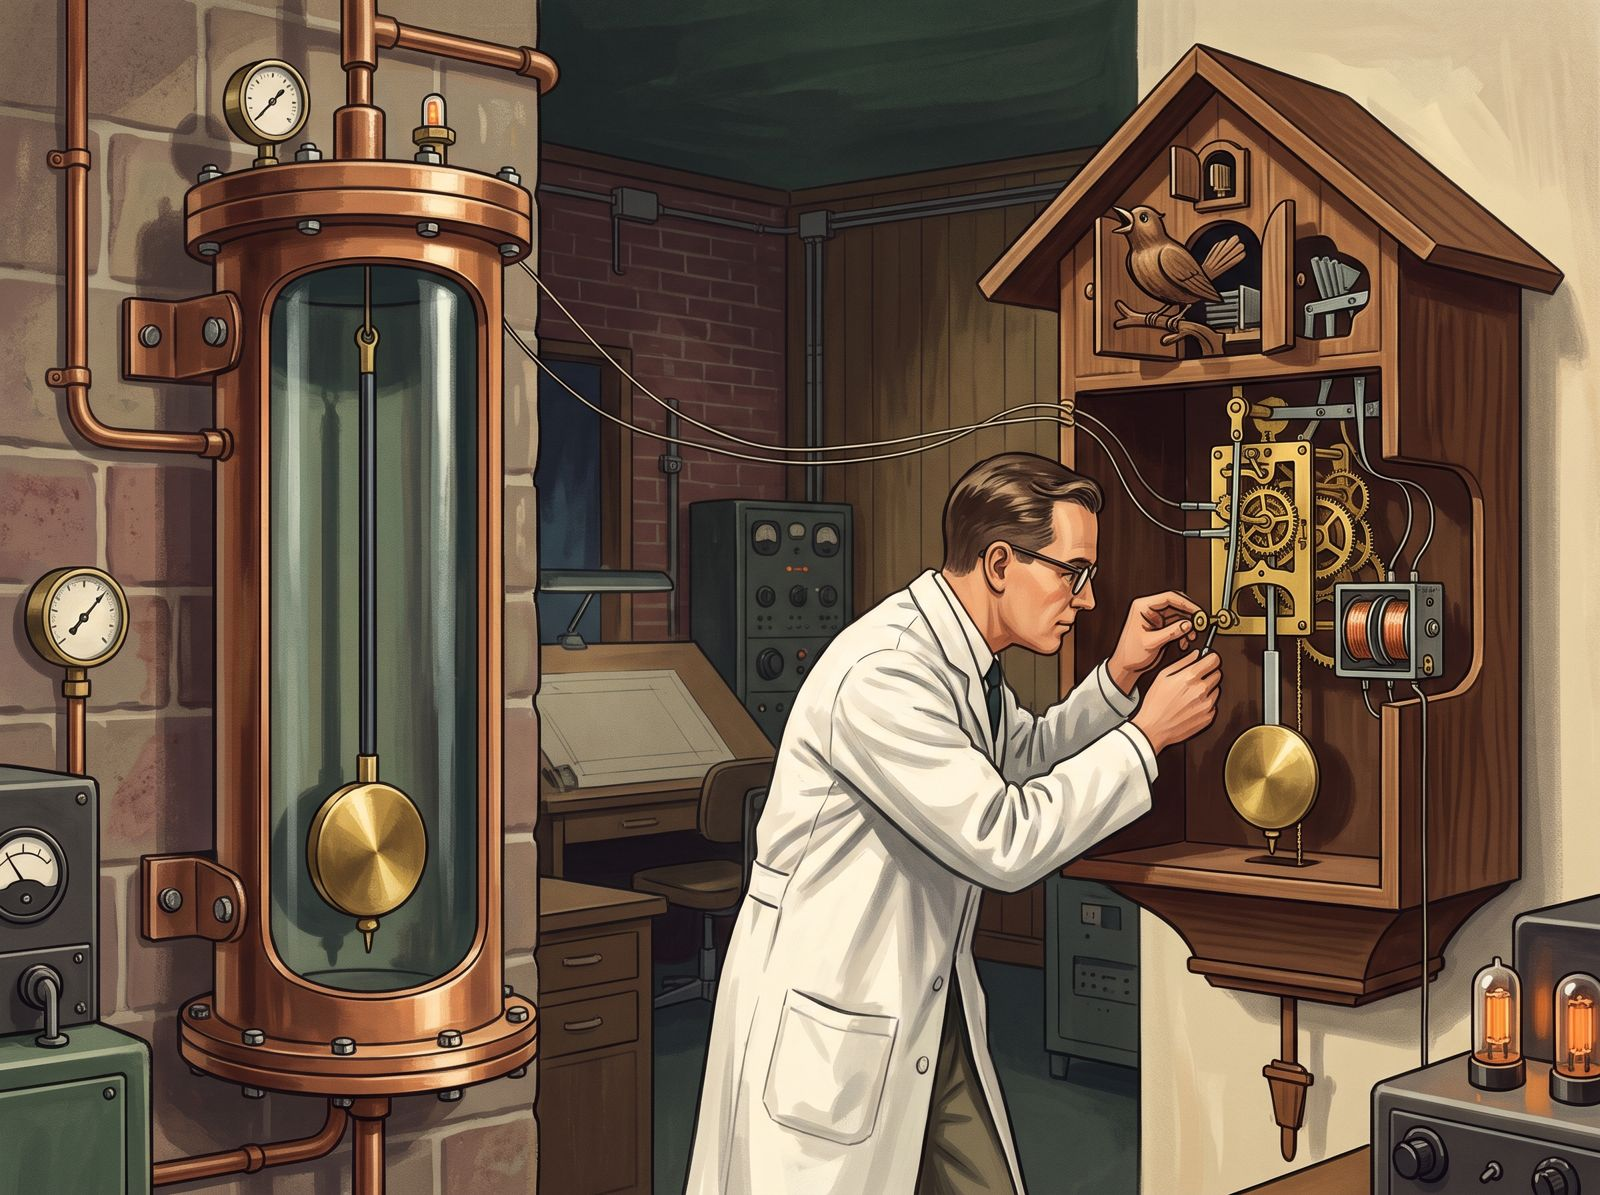
\includegraphics[width=0.8\textwidth]{shortt-master-and-slave.jpg}
  \caption{The Shortt arrangement: a free master pendulum in its vacuum tank, and the slave
    pendulum driving the cuckoo. \textit{(Illustration.)}}
\end{figure}

\section{Practical requirements}

Four requirements must be settled in the first weeks, before any subsystem design is frozen.

\begin{itemize}
  \item \lead{Budget and sourcing:} a parts list with a fallback for every hard-to-find item.
    Blank 80-column cards are scarce, so plan to cut cards from card stock of the right
    thickness. A working Model 33 can take months to find; identify a machine or donor early
    and budget for restoration parts.
  \item \lead{Safety:} guards and an interlock on the punch dies, inspection of the Teletype's
    mains wiring before power-up, and enclosure of the Nixie high-voltage supply. A lockout
    procedure for each is signed off before students work on them unsupervised.
  \item \lead{Measurement setup:} a time-interval counter or logic analyzer timestamps the
    pendulum's optical gate against GNSS PPS. Every timing criterion depends on this
    instrument, so it must be in hand before integration starts.
  \item \lead{AI-use policy:} prompts, model versions, and translation outputs are logged for
    every build, and credit for translated code is documented in the final report. The failed
    translations, and what the differential tests caught, are a project result in their own
    right and suitable for a conference poster or paper.
\end{itemize}

\section{Learning outcomes}

By the end of the project, students will be able to:

\begin{enumerate}
  \item Specify, document, and test interfaces between subsystems built by teams from other
    disciplines.
  \item Design and tune a feedback control loop that steers a physical oscillator to an
    external time reference, including holdover behavior.
  \item Use GNSS timing (PPS, NMEA/UBX messages) and characterize timing error with measured
    data.
  \item Critically evaluate AI-generated code through differential testing, rather than
    accepting it on inspection.
  \item Design a data encoding with error detection for a physical storage medium.
  \item Build precision electromechanical actuators and sensors, including solenoid or stepper
    actuation and optical sensing.
  \item Run a staged integration plan with defined fallback paths when a subsystem slips.
\end{enumerate}

These map onto the ABET student outcomes for complex problem solving, design, communication,
teamwork, and experimentation.

\begin{figure}[!htbp]
  \centering
  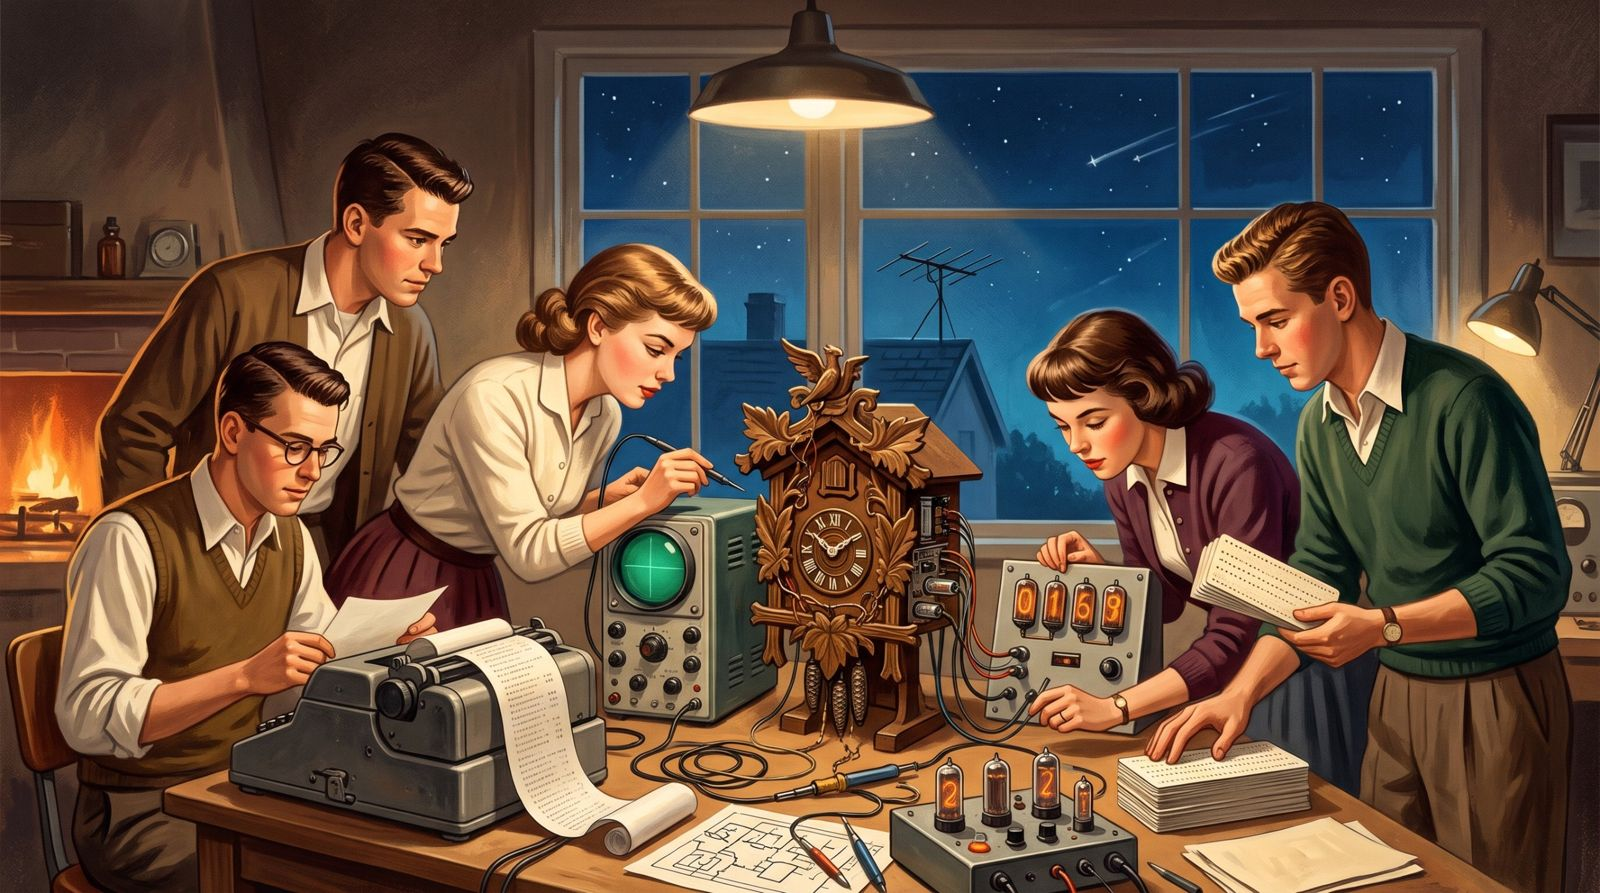
\includegraphics[width=0.8\textwidth]{integration-night.jpg}
  \caption{Integration night: oscilloscope, Teletype log, Nixie display, and the card deck
    all checked against the sky. \textit{(Illustration.)}}
\end{figure}

\section{Deliverables, milestones, and evaluation}

The full chain must run end to end by mid-spring, leaving the second half of the year for
timing measurements and the final demonstration.

\begin{figure}[!htbp]
\centering
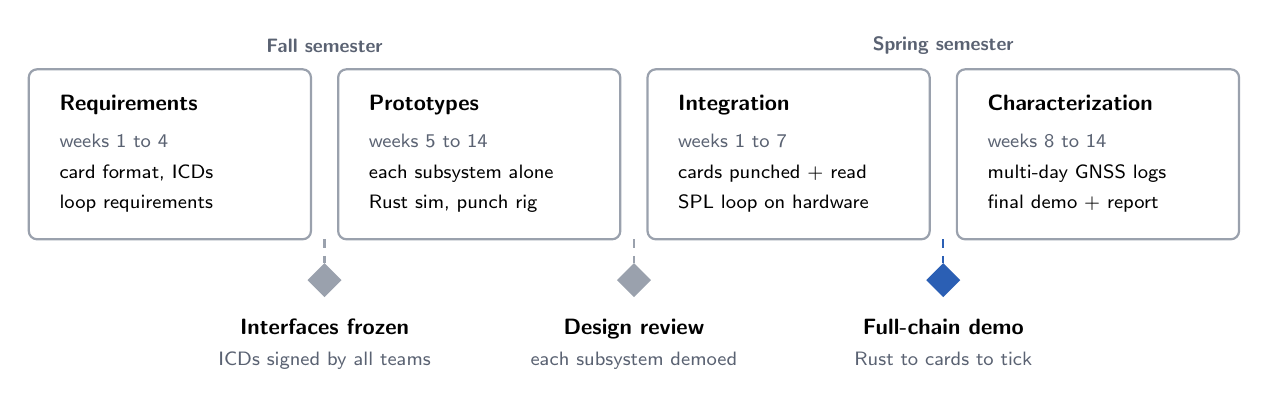
\begin{tikzpicture}[dia]
  \node[font=\sffamily\scriptsize\bfseries, text=quiet] at (198,62) {Fall semester};
  \node[font=\sffamily\scriptsize\bfseries, text=quiet] at (562,62) {Spring semester};
  \foreach \x/\t/\w/\a/\b in {
      24/Requirements/weeks 1 to 4/{card format, ICDs}/loop requirements,
      206/Prototypes/weeks 5 to 14/each subsystem alone/{Rust sim, punch rig},
      388/Integration/weeks 1 to 7/cards punched + read/SPL loop on hardware,
      570/Characterization/weeks 8 to 14/multi-day GNSS logs/final demo + report} {
    \draw[box] (\x,76) rectangle ++(166,100);
    \node[anchor=base west, font=\sffamily\footnotesize\bfseries] at (\x+12,100) {\t};
    \node[anchor=base west, note] at (\x+12,122) {\w};
    \node[anchor=base west, font=\sffamily\scriptsize] at (\x+12,140) {\a};
    \node[anchor=base west, font=\sffamily\scriptsize] at (\x+12,158) {\b};
  }
  \foreach \x/\c/\t/\s in {
      198/axis/Interfaces frozen/ICDs signed by all teams,
      380/axis/Design review/each subsystem demoed,
      562/accent/Full-chain demo/Rust to cards to tick} {
    \draw[\c, dashed, line width=0.8pt] (\x,176) -- (\x,190);
    \fill[\c] (\x,190) -- ++(10,10) -- ++(-10,10) -- ++(-10,-10) -- cycle;
    \node[anchor=base, font=\sffamily\footnotesize\bfseries] at (\x,232) {\t};
    \node[anchor=base, note] at (\x,250) {\s};
  }
\end{tikzpicture}
\caption{Two-semester schedule: four phases and three gates. The gates keep the chain from
  slipping into spring.}
\label{fig:schedule}
\end{figure}

The full-chain demo is the critical gate. If the punch or reader slips, teams fall back to a
hand-punched short deck or a serial stand-in for the reader so the controller and movement
can still be integrated on schedule.

\begin{table}[!htbp]
\small
\begin{tabularx}{\textwidth}{@{}Y L{1.4in} L{1.2in}@{}}
\toprule
\sffamily\bfseries Deliverable & \sffamily\bfseries Owner & \sffamily\bfseries Due at \\
\midrule
Rust reference firmware and simulator & CS & Design review \\
AI translator and differential test harness & CS & Design review \\
Card encoding spec and working punch & Mechatronics & Design review \\
Card reader with checksum validation & EE & Full-chain demo \\
Controller board with SPL runtime and I/O shim & EE, CS & Full-chain demo \\
Disciplined cuckoo movement & Mechatronics, EE & Full-chain demo \\
Final report, timing data, public demo & All & End of spring \\
\bottomrule
\end{tabularx}
\caption{Deliverables, owners, and the gate each is due at.}
\label{tab:deliverables}
\end{table}

Proposed evaluation criteria, with numeric targets to be set by the faculty sponsor at
kickoff:

\begin{itemize}
  \item \lead{Timekeeping:} clock time offset from GNSS over a multi-day run, and drift during
    a planned GNSS outage.
  \item \lead{Translation correctness:} SPL output matches the Rust reference on every
    recorded test vector.
  \item \lead{Media integrity:} the full deck reads with no uncorrected errors across repeated
    passes.
  \item \lead{Function:} the cuckoo calls the correct count on every hour of the test run.
  \item \lead{Engineering process:} interface documents kept current, design reviews passed,
    individual contributions documented.
\end{itemize}

\vfill
{\color{rule}\rule{\textwidth}{0.6pt}}\par
{\sffamily\footnotesize\color{quiet}
Text drafted with AI assistance (Claude, Anthropic); review by Nathaniel Frissell, W2NAF, is
in progress. Illustrations generated with Google Gemini; they are artistic depictions, not
drawings of the actual build.\par
A project of the University of Scranton Amateur Radio Club (W3USR).
\url{https://github.com/w3usr/gnss-cuckoo-clock}. Text licensed CC BY 4.0.\par}

\end{document}
